\documentclass{article}
\usepackage{v-equation}
\usepackage{pgfplots}
\geometry{
paperwidth=5in, 
paperheight=5in, 
top=10mm, 
bottom=10mm, 
left=10mm, 
right=10mm
}

\begin{document}
\begin{center}
Absorption of X-rays
\end{center}
\vspace*{\fill}
\begin{center}
\begin{tikzpicture}
	\draw[pattern, pattern=north east lines] (0, 0) rectangle (1.5, 3);
	\tzline[|<->|]<0, -0.25>(0, 0)(1.5, 0){$t$}[b, midway]
	\tzsnake[->][post length=20pt]<-2, 0.5>(0, 0)(2, 0)
	\tzsnake[->][post length=20pt]<-2, 1.5>(0, 0)(2, 0)
	\tzsnake[->][post length=20pt]<-2, 2.5>(0, 0)(2, 0)
	\tzsnake[->][post length=20pt]<1.5, 0.5>(0, 0)(2, 0)
	\tzsnake[->][post length=20pt]<1.5, 1.5>(0, 0)(2, 0)
	\tzsnake[->][post length=20pt]<1.5, 2.5>(0, 0)(2, 0)
	\node at (-2, 1.5)[left] {$I_0$};
	\node at (4, 1.5)[left] {$I$};
\end{tikzpicture}
\end{center}
\vspace*{\fill}
{\LARGE{
\begin{align*}
I = I_0e^{-\alpha t}
\end{align*}
}}
\vspace*{\fill}

\pagebreak
\vspace*{\fill}
\begin{equation*} 
\eqnmarkbox[blue]{node1}{I} =
\eqnmark[red]{node2}{I_0} e^{
\eqnmark{node3}{-\alpha } \eqnmark{node4}{t}}
\end{equation*}
\annotate[yshift=1em]{left}{node1}{intensity of emergent X-rays} 
\annotate[yshift=-0.5em]{below,left}{node2}{intensity of incident X-rays} 
\annotate[yshift=-1em]{below}{node3}{absorption coefficient of the material}
\annotate[yshift=1em]{right}{node4}{thickness of the material}

\vspace*{\fill}

\begin{center}
	\fbox{\qrcode[link, height=2cm]{http://www.ctan.org}}
\end{center}

\pagebreak
\begin{center}
\begin{tikzpicture} 
\begin{axis}[
	hide axis,
    axis equal,
    axis lines=middle,
    axis line style={->},
    tick style={color=black},
    xtick=\empty,ytick=\empty,
]
    \addplot [samples=10, domain=0:0.5*pi,->,
        % the default choice 'variable=\x' leads to
        % unexpected results here!
        variable=\t,
        quiver={
            u={-sin(deg(t))},
            v={cos(deg(t))},
            scale arrows=0.15,
        },
    ] ( {cos(deg(t))}, {sin(deg(t))} );
    \addplot [
        samples=100, domain=0:2*pi,
    ] ( {cos(deg(x))}, {sin(deg(x))} );
\end{axis}
\tzdot*(0, 0)
\end{tikzpicture}
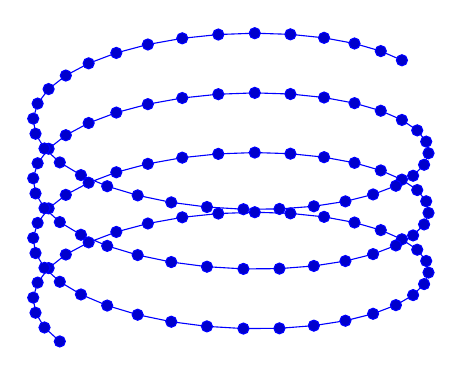
\begin{tikzpicture} 
\begin{axis}
[hide axis, view={60}{30}]
    \addplot3+ [
        domain=-pi:6*pi,
		samples=120,
		samples y=0,
	](
        {sin(deg(x))},
        {cos(deg(x))},
        {2*x/(5*pi)}
    );
\end{axis}
\end{tikzpicture}
\begin{tikzpicture} 
\begin{axis}[
	hide axis,view={0}{90},
    samples=10,
    z buffer=sort,
]
    %\addplot3 [surf]
     %   ({x*cos(deg(y))},{x*sin(deg(y))},{x});
    \addplot3[mesh, draw=black] table [x index=0,y index=1,z index=2,header=false] {sphere.dat};
\end{axis}
\end{tikzpicture}
%\tikz \addplot3 table [x index=0,y index=1,z index=2,header=false] {sphere.dat};
%\tikz \draw plot[smooth] file {sphere.table};
\begin{tikzpicture} \begin{axis}
    \addplot shell [
        prefix=pgfshell_,
id=cos, const plot]{
        awk 'BEGIN{
            pi=3.14159; N=10;
            for(i=0;i<=N;i++) print i,cos(i/N*pi);
        }'
    };
\end{axis}
\end{tikzpicture}
\begin{tikzpicture} 
\begin{axis}
	%[hide axis]
    \addplot shell [
        prefix=pgfshell_,
		id=sin,
		mark size=1pt,
		]{
        awk 'BEGIN{
            pi=3.14159; N=2*pi;
            for(i=0;i<=N;i+=0.1) print i,sin(i);
        }'
    };
\end{axis}
\end{tikzpicture}

\begin{tikzpicture} 
\begin{axis}
	[hide axis, width=10cm, height=12cm]
    \addplot3 shell [
        prefix=pgfshell_,
		id=helix,
        only marks,
		mark options={
        		scale=1.5,
        		fill=black,
        		draw=black,},
		smooth
		]{
        awk 'BEGIN{
            pi=3.14159; N=12*pi;
            for(i=0;i<=N;i+=0.1) print sin(i),cos(i), i;
        }'
    };
\end{axis}
\end{tikzpicture}
\end{center}
\pagebreak

\vspace*{\fill}
\begin{center}
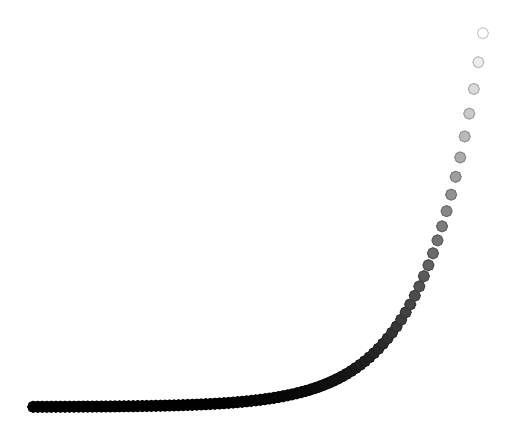
\begin{tikzpicture} 
\begin{axis}[
	hide axis,
    colormap={bw}{
        gray(0cm)=(0);
        gray(1cm)=(1);
    },
]
\addplot+ [
        scatter,
        only marks,
        domain=0:8,
        samples=100,
    ] {exp(x)};
\end{axis}
\end{tikzpicture}
\end{center}
\vspace*{\fill}

\pagebreak

\vspace*{\fill}
\begin{center}
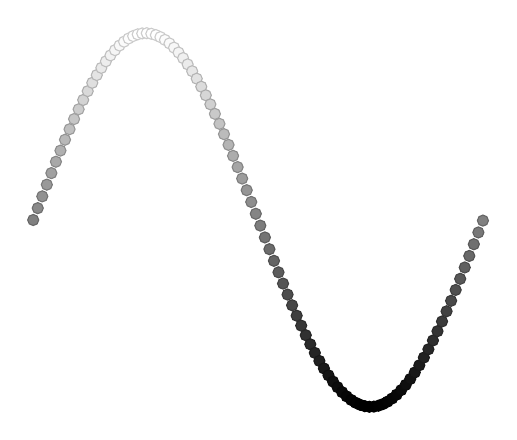
\begin{tikzpicture} 
\begin{axis}[
	hide axis,
    colormap={bw}{
        gray(0cm)=(0);
        gray(1cm)=(1);
    },
]
\addplot+ [
        scatter,
        only marks,
        domain=0:6.28,
        samples=100,
    ] {sin(deg(x))};
\end{axis}
\end{tikzpicture}
\end{center}
\vspace*{\fill}

\pagebreak
\vspace*{\fill}
\begin{center}
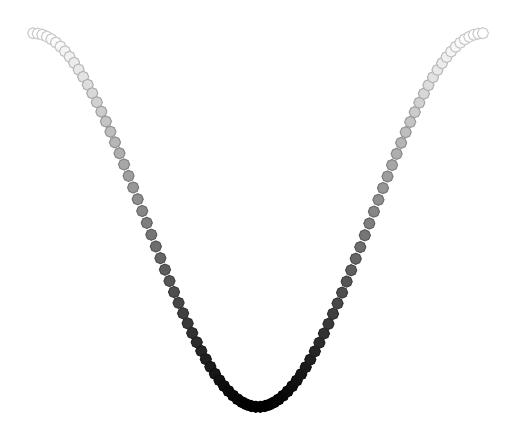
\begin{tikzpicture} 
\begin{axis}[
	hide axis,
    colormap={bw}{
        gray(0cm)=(0);
        gray(1cm)=(1);
    },
]
\addplot+ [
        scatter,
        only marks,
        domain=0:6.28,
        samples=100,
    ] {cos(deg(x))};
\end{axis}
\end{tikzpicture}
\end{center}
\vspace*{\fill}

\pagebreak
\vspace*{\fill}
\begin{center}
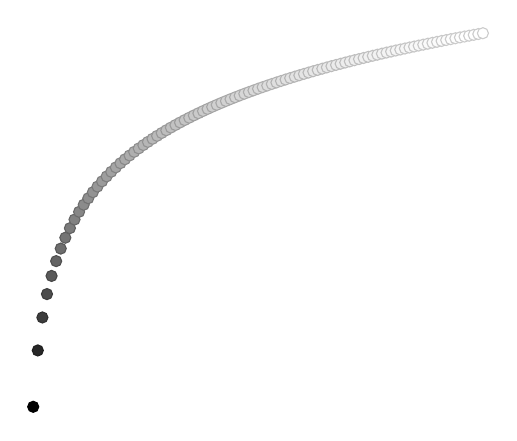
\begin{tikzpicture} 
\begin{axis}[
	hide axis,
    colormap={bw}{
        gray(0cm)=(0);
        gray(1.5cm)=(1);
    },
]
\addplot+ [
        scatter,
        only marks,
        domain=0:8,
        samples=100,
    ] {ln(x)};
\end{axis}
\end{tikzpicture}
\end{center}
\vspace*{\fill}
\end{document}
